\chapter{Clustering-based Matrix Factorization for Online Shopping Prediction}
\label{chp:cbmf}
\section{Limitation of TRIMF}
In Chapter \ref{chp:trimf}, we introduced TRIMF, which is a matrix tri-factorization method for cross-domain recommendation. However, it has some limitations which restrict its scalability and extensibility. First, when data are coming from multiple sources (e.g. click, pageview and add cart), TRIMF treats every source equally and puts each of them into a matrix which is very sparse. When solving the object function, increasing the matrixes will increase the time and space complexity. If we try to update $S$, every matrix is included so it will be quite time-consuming. What is more, in reality we cannot ignore users with fewer actions. Thus, the matrix will be much more sparse than the ones in our experiment, so we cannot guarantee achieving equal performance.

To solve these problems, we have developed a framework based on a clustering and scoring scheme (CBMF, Figure \ref{fig:cbmf}). CBMF first clusters users according to their behaviors and demographic features, then automatically converts different types of actions into one matrix, called action matrix. Finally a matrix factorization method is applied to the action matrix. For users with adequate actions, a personalized recommendation is provided. Otherwise we provide a recommendation based on their clusters.

We conduct two experiments: 
\begin{itemize}
\item offline experiment: we select datasets used in TRIMF, and compare the run-time and precision of the two methods.
\item online experiment: we do A/B test with CBMF in an online shopping site.
\end{itemize}
Results show that in offline datasets, CBMF runs much faster then TRIMF while achieving equal performance. In online test, CBMF outperforms other methods in conversion rate.


\begin{figure}

%\begin{Large}

\begin{center}
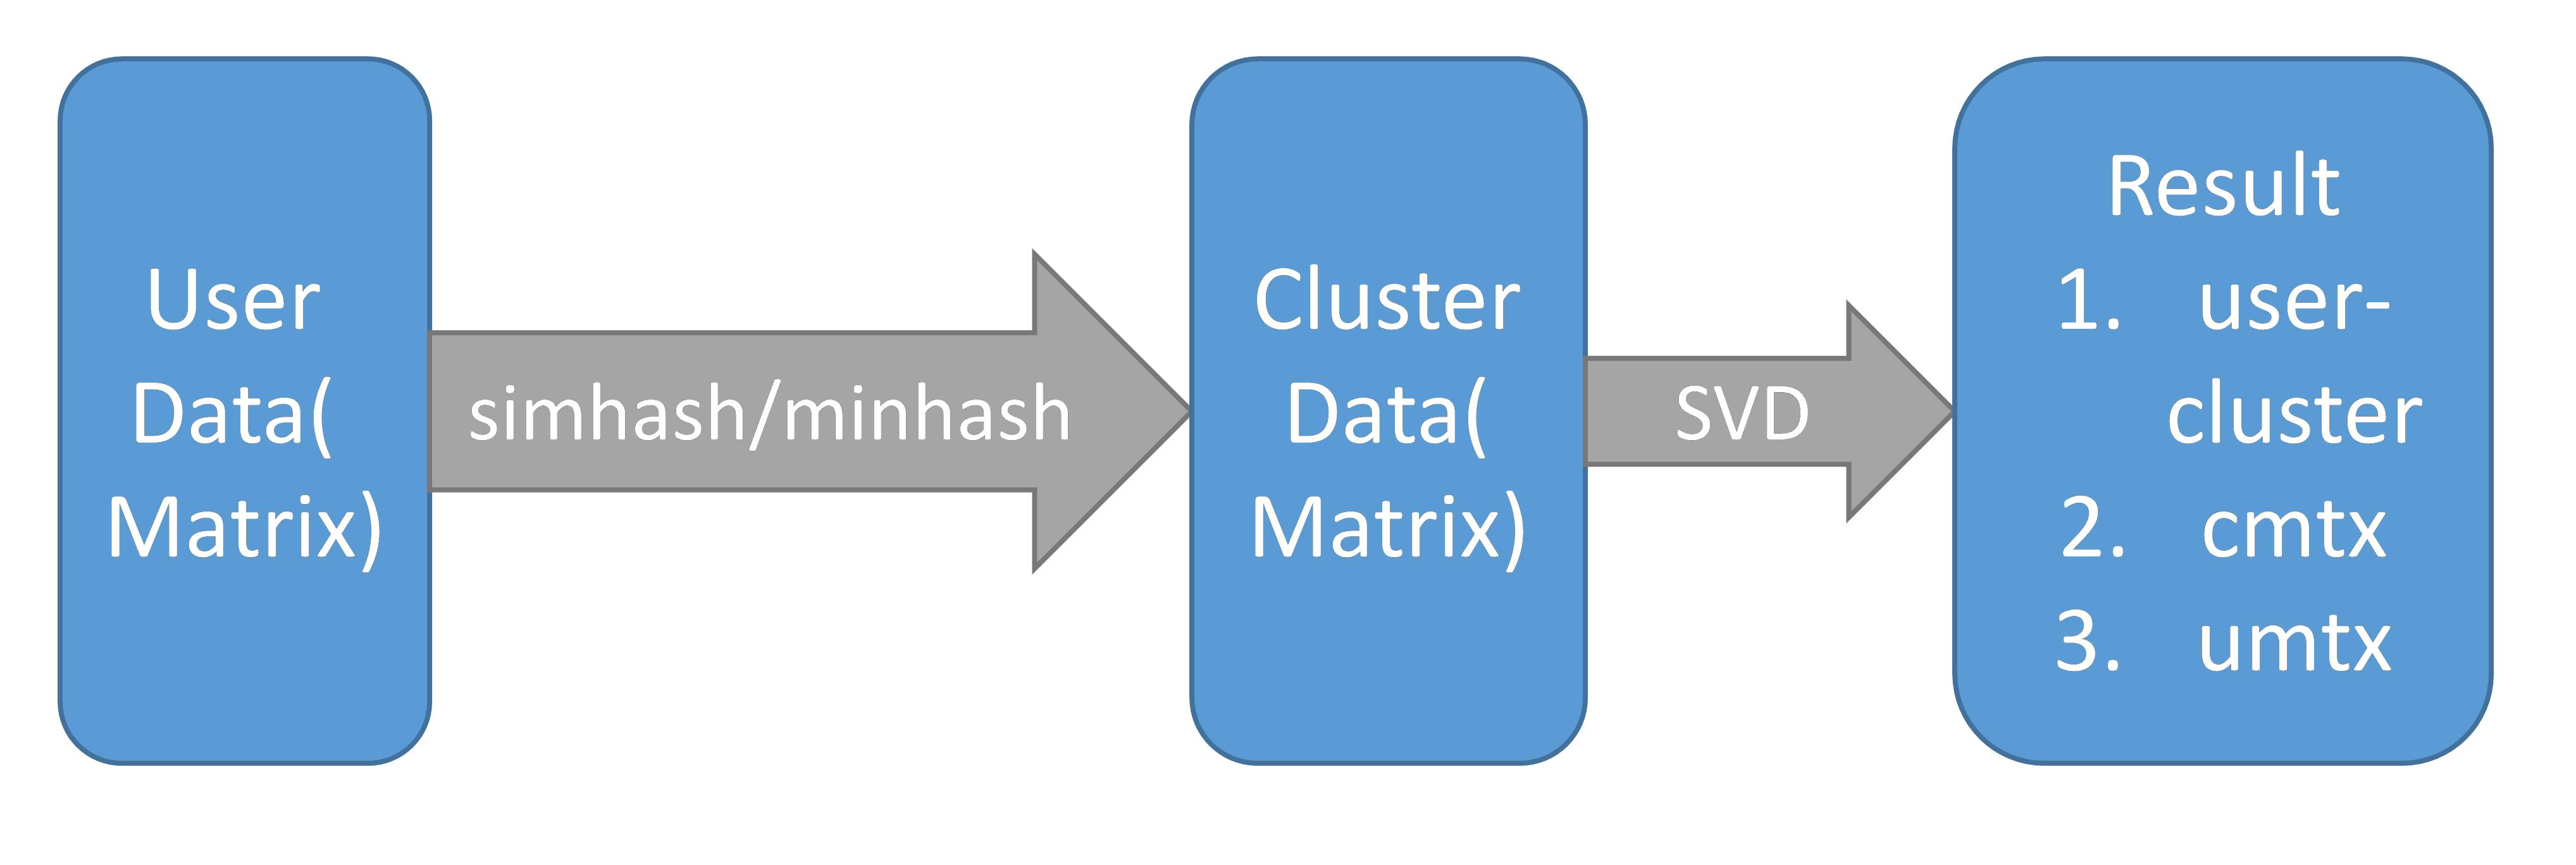
\includegraphics[width=400px]{fig/d} 
\caption{Framework of CBMF.}
\label{fig:cbmf}
\end{center}
\end{figure}





\section{Clustering Method in CBMF}

Usually users’ actions are unique and sparse and it would be time-consuming if we want to cluster users by using raw data. In Tencent, we have 800,000,000 users in total, and their feature vectors dimensions can be as large as 1,000,000. Therefore, if we want to speed up the phase, we must first convert large sparse user vector into a low dimensionally dense vector.

\subsection{Simhash}

Simhash is a kind of locality sensitive hashing(LSH). LSH is a hashing method where if we got two points $A,B$ which are close in their original space, after hashing we would get $A',B'$, with $A',B'$ still close in the new space. Thus we keep the relationship of distance among the two spaces. 

The input of Simhash per user is $(feature_1, weight_1),..(feature_n,weight_n)$. The procedure of Simhash is in Algorithm \ref{algorithm:simhash}.

\begin{algorithm}[tb]
\caption{Simhash Algorithm for one instance.}
\begin{algorithmic}

\STATE {\bfseries Input:} $\X_U$, $h$\\
$\X_{U}$ : $(feature_1, weight_1),..(feature_n,weight_n)$ \\
$h$: a smooth hash function with $k$ bits after hashing\\

\STATE {\bfseries Initialize:} $r$(result vector) : $[0,0,0..0] \in \{0,1\}^k$

\FOR{ $i$ = 1 to $n$}

\STATE calculate $h(feature_i)$

\STATE $r = r + weight_i * h(feature_i)$

\ENDFOR

\FOR{ $i$ = 1 to $k$}
\IF {$r_i > 0$}
\STATE {$r_i = 1$}
\ELSE 
\STATE {$r_i = 0$}
\ENDIF
\ENDFOR

\STATE {\bfseries Output:} $r$

\end{algorithmic}
\label{algorithm:simhash}
\end{algorithm}

Assume that Simhash converts a vector $x$ into a 32-dimension binary vector $x'$. Actually $i_{th}$ bit of $x'$ is the sign of the inner product of $x$ and $H_i = [h^1_i, h^2_i,...h^n_i]$, $H_i$ can be regarded as a hyperplane in original space. If two vectors $x, y$ are in the same direction of $H_i$, then $x', y'$ is equal on $i_{th}$ bit. Thus we can use hamming distance in the new space to represent their similarity in original space.

\subsection{Minhash}

The similarity between two users $u_i , u_j$ is defined as the overlap between their item sets. $S(u_i, u_j) = \frac{C_{u_i} \cup C_{u_j}}{C_{u_i} \cap C_{u_j}}$, also known as the Jaccard coefficient. Regardless, calculating all similarities in real-time is nearly impossible. However, we can achieve a provably sublinear time near-neighbor search technique by applying Minhash.

MinHash is a probabilistic clustering method that assigns a pair of users to the same cluster with a probability proportional to the overlap between the set of items that these users have voted for (clicked-on). In CBMF, Minhash is applied after Simhash and every user vector consists of 32 bits. 

The basic idea in the Minhash scheme is to randomly permute the set of items (S) and for each user $u_i$ compute its hash value $h(u_i)$ as the index of the first item under the permutation that belongs to the user’s item set $C_{u_i}$. It is also easy to prove that the probability of two users having the same hash function is exactly equal to their similarity or Jaccard coefficient.Similar to \cite{Indyk:1998:ANN:276698.276876}, we can always concatenate $p$ hash-keys for
users, where $p \ge 1$, so the probability that any two users $u_i , u_j$ will agree the concatenated hash-key is equal to $S(u_i , u_j )^p$. In that case, $p$ can be a parameter to control the number of clusters. If $p$ is large, then the clusters will be more refined thus the number of clusters will increase.

\subsection{Simhash \& Minhash using MapReduce}

MapReduce is a model of computation over large clusters of machines that can handle processing of large amounts of data in relatively short periods of time and scales well with the number of machines. Our method Simhash and Minhash can easily be implemented using hadoop.

\subsubsection{Map phase}
In the map phase, we read the input records independently, in parallel, on different machines and map each input to a set of key-
value pairs. In our case, hadoop streaming is applied and each input instance is a user's vector(in sparse representation).

We first iterate the user's vector $u_i$, using Simhash to convert the vector to a 32-bit binary vector, the hashing function used in Simhash is FNV-32. Then Minhash is applied $p$ times per user. We concatenate the $p$ Minhash values $Mnhs_i$ to obtain the cluster id of the user. Finally, the output is ( $Mnhs_i$, $u_i$), key is $Mnhs_i$, value is $u_i$. For users with enough actions, we output another pair ( $user-id$, $u_i$). 

\subsubsection{Reduce phase}

In the reduce phase, our input takes two forms: ($Mnhs_i$, $u_i$) represents cluster-id and user vector. ($user-id$, $u_i$) represents an experienced user and his vector.
\begin{itemize}
\item In the cluster case: for each cluster-id we obtain the list of user-ids that belong to this cluster and prune away clusters with members less than 10. For each cluster-id, a joint vector is needed to represent all users in it. Thus we simply add scores from users to the joint vector. We, then do a normalization sothe range of the vector is between 0 and 1. The output has two parts: 
\begin{itemize}
\item users and the cluster they belong to (userid, clusterid). 
\item cluster-ids and their vectors (cluster-id, cluster-vector).
\end{itemize}
\item In the user case: we simply output the normalized vector.

\end{itemize}

After the reduce phase, we have three tables(matrices). 1, user and the respective cluster-id; 2, cluster-id and its vector; 3, user and respective vector.

\section{Feature Construction in CBMF}

After clustering, we have many clusters and their corresponding actions, including click, purchase and pageview on different (overlapping) items.

The naive way to handle those actions is to create a matrix $X_i$ for each action $i$. In matrix $X_i$, a row represents a cluster while a column represents an item, $X_{mn}$ represents the frequency of action that users in cluster $m$ used on item $n$. However, simply creating such a matrix may lead to data sparsity problems. This is especially true in the matrix standing for purchasing actions, even though similar users are alredy clustered together.The data is still very sparse($0.01\%$) which may constrain our model from providing a reasonable recommendation.

In CBMF, a scoring scheme is applied for each kind of action to put every action into a single matrix with a proper score. For a specific item, a user may have four kinds of actions (click, purchase, pageview and uninterested). The idea behind the construction is that for a specific goal (e.g predict future purchase), the score that should be given to an action depends on how much impact the action can have.

For example, if we want to improve conversion rate, let $U_n$ denote the users who bought item $n$, while $U$ denotes the entire user set. The average conversion rate for a given item $n$ can be approximated by $Cvr(n_{all}) \approx \frac{|U_n|}{|U|}$. 
For a given action(e.g. click), let $U_n^{click}$ denote the users who clicked item $n$. Then the conversion rate for users who had clicked these items can then be approximated by $Cvr(n_{click}) \approx \frac{|U_n \cap U_n^{click}|}{|U_n^{click}|}$we compare the conversion rate of users with this action with the average, and their log ratio $log(\frac{Cvr(n_{click})}{Cvr(n_{all})})$ is our initial score.

For each action with an item we calculate a score, in CBMF we use weighted scores and add them together. That is, for cluster $m$ and item $n$, if we have four scores:$s_1, s_2, s_3, s_4$ and their corresponding weights:$w_1, w_2, w_3, w_4$. $w_i$ is the percentage of users who have this action compared to all users. The result, $X_{mn} = \frac{\sum_{i=1}^4 w_i*s_i}{\sum_{i=1}^4 w_i}$. 

\section{Matrix Factorization in CBMF}

Once the matrices are generated, we use Singular Value Decomposition(SVD) from mahout \footnote{https://mahout.apache.org/users/dim-reduction/dimensional-reduction.html}. The number of eigenvalues is set to 20 according to the online test.

After SVD, we can provide recommendations to every user; for experienced users direct results are provided, otherwise we find the user's cluster-id and provide results for this cluster as our recommendation. We output our results to an online key-value dataset called TDE. Once a user comes, we search his id in TDE, and the return value is our recommendation.


